\section{Theorie}
\label{sec:Theorie}

\subsection{Relaxationsverhalten des RC-Kreises}
    Zwischen den Platten eines Kondesators liegt die Spannung 
    \begin{equation}
        \label{eq:sp}
        U_C = \dfrac{Q}{C}
    \end{equation} an.
    Beim Ausgleich der Ladungen, sprich der Entladung des Kondensators entseht der 
    Strom 
    \begin{equation}
        \label{eq:st}
        I = \dfrac{U_C}{R}.
    \end{equation}
    Aus dem Zusammenhang $dQ=-I\ dt$ kann durch Einsetzen von \ref{eq:sp} und \ref{eq:st}
    die Differentialgleichung 
    \begin{equation}
        \dfrac{dQ}{dt}= -\dfrac{1}{RC} Q{t}
    \end{equation}
    gewonnen werden. Der Entladevorgang lässt sich offensichtlich durch 
    \begin{equation}
        \label{eq:dgl}
        Q(t)=Q(0)e^{\dfrac{-t}{RC}}
    \end{equation}
    beschreiben. Der die DGL ebenfalls lösende Term mit positivem Exponenten entfällt aufgrund der 
    Bedingung $Q(\infty)=0$.\\
    Für den Aufladevorgang gilt die gleiche Differentialgleichung \ref{eq:dgl}. Ledeglich die
    Randbedingungen lauten nun $Q(0)=0$ und $Q(\infty)=CU_0$. Unter diesen Bedingungen lässt sich 
    die Differentialgleichung durch 
    \begin{equation}
        Q(t) = CU_0(1-e^{\dfrac{-t}{RC}})
    \end{equation}
    lösen.\\
    Die Zeitkonstante RC ist ein Maß für die Relaxationsgeschwindigkeit. Während des 
    Zeitintervalls $\Delta T=RC$ sinkt die Ladung des Kondensators um den Faktor
    $\dfrac{Q(t=RC)}{Q(0)}=\dfrac{1}{e}$.

\subsection{Relaxationsverhalten unter Einfluss angelegter periodischer Spannung}
    Ist die Frequenz der angelegten Wechselspannung $U(t)=U_0\cos{\omega t}$ sehr niedrig,
    so verhält sich $U_C(t)$ wie $U(t)$. Bei höheren Frequenzen verzögert sich 
    die Auf- und Entladung des Kondensators durch den Widerstand, sodass eine 
    Phasenverschiebung $\phi$ zwischen dem Kondensator und der Spannungsquelle 
    entsteht. Dadurch verringert sich auch die Amplitude der Kondensatorspannung.
    im folgenden wird für die Kondensatorspannung der Ansatz $U_C(t)=A(\omega)
    \cos{\omega t + \phi{\omega}}$ verwendet.
    \begin{figure}[H]
        \centering
        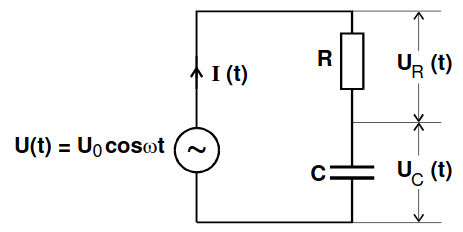
\includegraphics{schalt3.png}
        \caption{Der RC-Schaltkreis mit angelegter Cosinus-Spannung}
        \label{fig:schalt3}
    \end{figure}
    Die Spannung des in Abbildung \ref{fig:schalt3} dargestellten Stromkreises kann nach dem zweiten
    Kirchhoffschen Gesetzt durch 
    \begin{equation}
        \label{eq:kirsche}
        U(t)=U_R(t)+U_C(t) \Leftrightarrow U_0 \cos{\omega t}=I(t)R + 
        A(\omega)\cos{\omega t + \phi}
    \end{equation}
    bestimmt werden. Wird sich nun ernaut des Zusammenhangs $\dfrac{dQ}{dt}=-I$ und 
    Gleichung \ref{eq:sp} bedient, ergibt sich
    \begin{equation}
        U_0\cos{\omega t}=-A(\omega)\omega RC \sin{\omega t+\phi}+A(\omega)\cos{\omega t + \phi}
    \end{equation}
    Wird nun $\omega=\dfrac{\pi}{2}$ gesetzt, wird diese Gleichung zu 
    \begin{equation*}
        0 = -\omega RC \sin{\dfrac{\pi}{2} + \phi}+\cos{\dfrac{\pi}{2}+\phi}
    \end{equation*}
    Wird nun ausgenützt, dass $\sin{\phi + \dfrac{\pi}{2}}$, entsteht die Betiehung
    \begin{equation}
        \label{eq:phi}
        \phi(\omega)=\arctan{-\omega RC}
    \end{equation}
    zwischen Phase und verwendeter Frequenz. Nun wird der der Fall $\omega t + \phi = 
    \dfrac{\pi}{2}$ betrachtet. Es gilt
    \begin{align*}
        U_0 \cos{\dfrac{\pi}{2}-\phi}=-A(\omega)\omega RC\\
        \Leftrightarrow A(\omega)=-\dfrac{\sin{\phi}}{\omega RC}U_0
    \end{align*}
    Unter Verwendung von \ref{eq:phi} kann die Beziehung $\sin{\phi}=\dfrac{\omega RC}
    {\sqrt{1+\omega^2 R^2 C^2}}$ hergeleitet und in die Gleichung eingesetzt werden.
    Dadurch ergibt sich 
    \begin{equation}
        A(\omega)=\dfrac{U_0}{\sqrt{1+\omega^2 R^2 C^2}}
    \end{equation}
    Während kleine Frequanzen nur eine geringe Abweichung von der angelegten Spannung
    aufweisen, verschwindet die Amplitude für sehr große Frequenzen.
    RC-Glieder stellen also einen Tiefpass im elektrischen Schaltkreis dar.

\subsection{Der RC-Kreis als Integrator}
    Ein anderer möglicher Effekt des RC-Kreises ist die Integration der Spannung. Wir betrachten 
    erneut Gleichung \ref{eq:kirsche}.
    \begin{equation*}
        U(t)=U_R(t)+U_C(t)=I(t)R+U_C(t)=RC\dfrac{dU_C}{dt}+U_C(t)
    \end{equation*} 
    Falls nun $\omega \ll \dfrac{1}{RC}$ ist die Spannung $\vert U_C \vert \ll \vert U_R \vert$
    Näherungsweise ist dann 
    \begin{equation}
        U(t)=RC\dfrac{dU_C}{dt} \Leftrightarrow U_C(t)=\dfrac{1}{RC}\int_0^t U(t')dt'.
    \end{equation}
